% Created 2014-07-14 Mon 16:02
\documentclass[11pt]{article}
\usepackage[utf8]{inputenc}
\usepackage[T1]{fontenc}
\usepackage{fixltx2e}
\usepackage{graphicx}
\usepackage{longtable}
\usepackage{float}
\usepackage{wrapfig}
\usepackage{rotating}
\usepackage[normalem]{ulem}
\usepackage{amsmath}
\usepackage{textcomp}
\usepackage{marvosym}
\usepackage{wasysym}
\usepackage{amssymb}
\usepackage{hyperref}
\tolerance=1000
\author{Zeeshan Lakhani}
\date{\today}
\title{core}
\hypersetup{
 pdfkeywords={},
  pdfsubject={},
  pdfcreator={Emacs 24.3.1 (Org mode 8.3beta)}}
\begin{document}

\maketitle
\setcounter{tocdepth}{3}
\tableofcontents


\section{StarterKit}
\label{sec-1}
\subsubsection{org.zeeshanlakhani.midwestio.core}
\label{sec-1-0-1}
\subsubsection{Namespace declaration}
\label{sec-1-0-2}
\begin{verbatim}
(ns org.zeeshanlakhani.midwestio.core
  (:require [clojure.test.check :refer [quick-check]]
            [clojure.test.check.generators :as gen]
            [clojure.test.check.properties :as prop]
            [schema.core :as s]
            [schema-gen.core :refer [schema->gen]]
            [clojure.core.matrix :refer [transpose]]))
\end{verbatim}

\section{Composing Test Generators}
\label{sec-2}
\section{Who Am I?}
\label{sec-3}
\subsection{Zeeshan Lakhani}
\label{sec-3-1}
\subsubsection{programmer at Beatport/SFX/Arc90}
\label{sec-3-1-1}
\subsubsection{a lead organizer of Papers We Love - \href{https://twitter.com/papers_we_love}{@paperswelove}}
\label{sec-3-1-2}
\subsubsection{\href{https://twitter.com/zeeshanlakhani}{@zeeshanlakhani}}
\label{sec-3-1-3}
\subsubsection{\href{https://github.com/zeeshanlakhani}{github.com/zeeshanlakhani}}
\label{sec-3-1-4}
\subsubsection{what I listened to while preparing this talk}
\label{sec-3-1-5}

\includegraphics[width=.9\linewidth]{../images/listen.jpg}
\url{http://bit.ly/U2FUpx}
\section{What We'll Cover}
\label{sec-4}
\subsection{Background - Tests, Property-Based-Testing}
\label{sec-4-1}
\subsection{Generation from a Data Validation Layer}
\label{sec-4-2}
\begin{itemize}
\item Prismatic Schema
\end{itemize}
\subsection{Case Study - Making My Job Easier}
\label{sec-4-3}
\subsubsection{More Definitive Talk on Property-Based-Testing - Jessica Kerr}
\label{sec-4-3-1}
\section{Where It All Starts\ldots{}}
\label{sec-5}

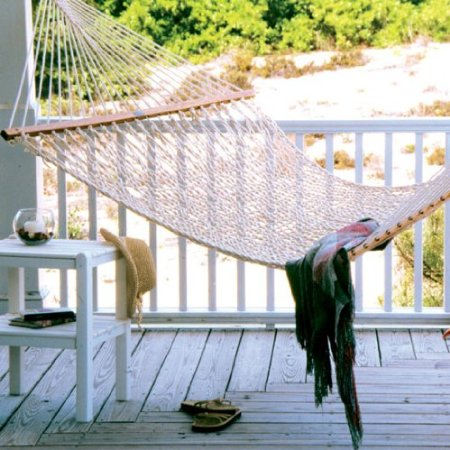
\includegraphics[width=.9\linewidth]{../images/hammock.jpg}
\url{http://www.amazon.com/Clojure-Bookshelf/lm/R3LG3ZBZS4GCT}
\section{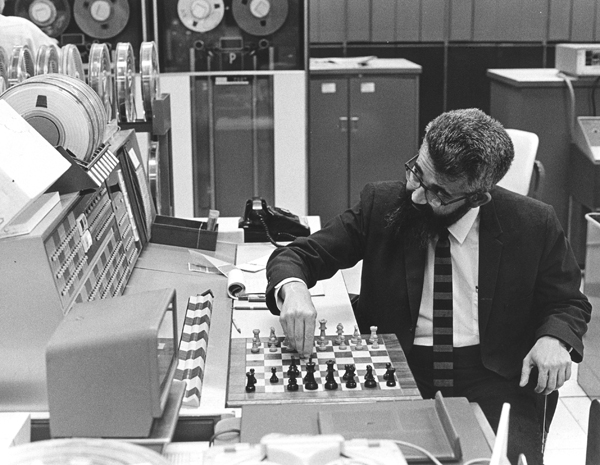
\includegraphics[width=.9\linewidth]{../images/mc.jpg}}
\label{sec-6}
\section{Beginnings}
\label{sec-7}


\includegraphics[width=.9\linewidth]{../images/artof.jpg}
\url{http://bit.ly/1zzylYo}
\section{\href{http://www.cs.tufts.edu/~nr/cs257/archive/john-hughes/quick.pdf}{Koen Claessen \& John Hughes}}
\label{sec-8}

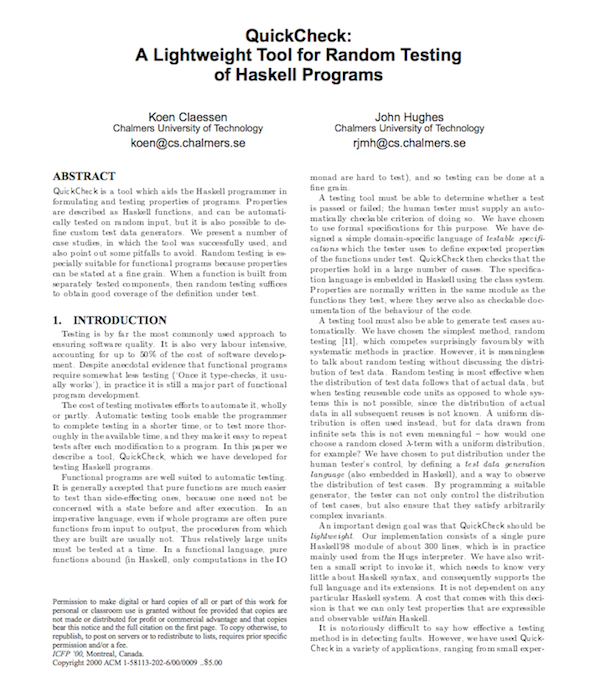
\includegraphics[width=.9\linewidth]{../images/qc_origin_go.png}
\url{http://bit.ly/1q8A7hn}
\section{\href{http://people.inf.elte.hu/center/fulltext.pdf}{Fun and Profit}}
\label{sec-9}

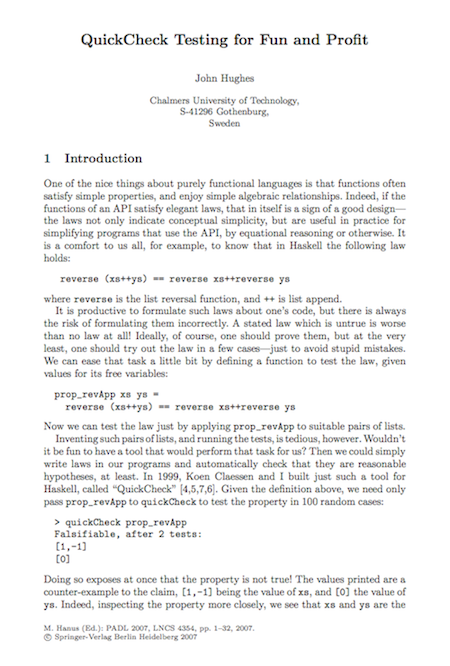
\includegraphics[width=.9\linewidth]{../images/qc_fun_go.png}
\url{http://bit.ly/1sbLMvz}
\section{\href{http://www.cse.chalmers.se/~nicsma/papers/finding-race-conditions.pdf}{More Recent - Erlang - PULSE}}
\label{sec-10}

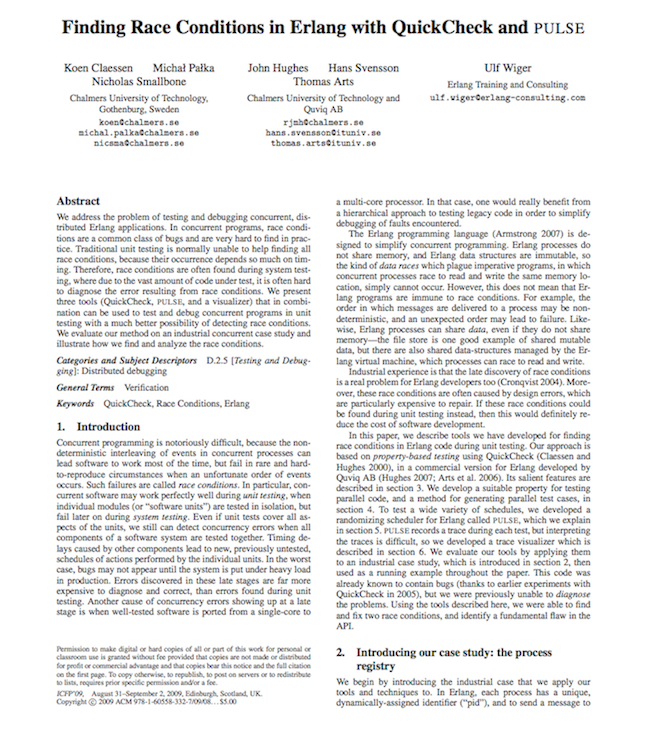
\includegraphics[width=.9\linewidth]{../images/qc_cond_go.png}
\url{http://bit.ly/1r923kA}
\section{From the Paper}
\label{sec-11}
\begin{quote}
We have designed a simple domain-specific language of
testable specifications which the tester uses to
define expected properties of the functions under test.
\end{quote}
\begin{quote}
We have chosen to put distribution under the human tester's
control, by defining a test data generation language\ldots{}
\end{quote}
\begin{quote}
We have taken two relatively old ideas, namely specifications
as oracles and random testing, and found ways to make them
easily available \ldots{}
\end{quote}
\section{The Idea}
\label{sec-12}
\begin{quote}
The idea of property-based testing is to write a specification
of the system under test in a suitable language, which is then
tested using a large collection of test data invented by the
computer
\end{quote}

\url{http://www.cse.chalmers.se/~nicsma/papers/lic.pdf}

\section{Why Do We Test and How?}
\label{sec-13}


\includegraphics[width=.9\linewidth]{../images/abt.png}
\url{http://unbounce.com/photos/abt2.png}

One Feature - O(n)
Pairs of Features - O(n\(^{\text{2}}\)) - quadratic
Triples of Features - O(n\(^{\text{3}}\)) - cubic
\section{Big Statement about Testing?}
\label{sec-14}


\includegraphics[width=.9\linewidth]{../images/dhh_go.jpg}
\url{http://bit.ly/1xRTmfg}
\section{This One, That One}
\label{sec-15}

\url{http://stackoverflow.com/a/17810004/413685}
\subsubsection{Dummy objects}
\label{sec-15-0-1}
are passed around but never actually used.
\subsubsection{Fake objects}
\label{sec-15-0-2}
actually have working implementations, but usually take some shortcut
which makes them not suitable for production (an in memory database
is a good example).
\subsubsection{Stubs}
\label{sec-15-0-3}
provide canned answers to calls made during the test\ldots{}
\subsubsection{Mocks}
\label{sec-15-0-4}
are objects pre-programmed with expectations which form a specification
of the calls they are expected to receive.
\subsubsection{testing(}
\label{sec-15-0-5}
Integration - Functional - Regression - Validation - Acceptance)
\section{Bias - Forgetful - Redundant - Tedious}
\label{sec-16}

\begin{verbatim}
;; Don't Run - Example

(deftest test-post
  (with-system
    (let [config (load-config)
          port (:http-server-port config)
          chart-to-create
          {:slug "foo-bar-baz"
           :name "Foo Bar Baz"
           :description {:en "foo"}
           :duration-seconds 100
           :created-by {:url "/accounts/brianolssen"}
           :media [{:url "/tracks/baby-monkey"} {:url "/videos/oh-my-dayum"}]}
          req {:accept :json
               :throw-exceptions false
               :content-type "application/json"
               :basic-auth ["brianolssen" "iF41ixXSUntFoXirPAXJ"]
               :body (json/encode chart-to-create)}
          path (route port :charts)]
      (testing "Post chart";; ...))))
\end{verbatim}
\section{Property-Based-Testing -> Establishing Invariants in Code}
\label{sec-17}
\section{Or Maybe A Better Title?}
\label{sec-18}
\section{\href{http://alexey.radul.name/ideas/2014/testing-revisited/}{Generating Circumstances}}
\label{sec-19}
\section{Examples}
\label{sec-20}
\section{Specification - The Transpose of a Transposed Matrix is the Original Matrix}
\label{sec-21}

(A\(^{\text{T}}\))\(^{\text{T}}\) = A

\begin{verbatim}
(def matrix-gen
  (gen/such-that
   not-empty
   (gen/vector
    (gen/tuple gen/int gen/int gen/int))))

(gen/sample matrix-gen 10)
\end{verbatim}

\begin{verbatim}
(def matrix
  [[1 2]
   [3 4]])

(transpose matrix)
\end{verbatim}

\begin{verbatim}
(def transpose-of-transpose-prop
  (prop/for-all [m matrix-gen]
  (= m (transpose (transpose m)))))

(quick-check 50 transpose-of-transpose-prop)
\end{verbatim}

\section{Failure \& Shrinking}
\label{sec-22}

\href{http://bit.ly/1kmjKFY}{Example From Clojure Cookbook}

\begin{verbatim}
(defn reciprocal-sum [s]
  (reduce + (map (partial / 1) s)))

(reciprocal-sum '(1 2))
\end{verbatim}

\begin{verbatim}
(def numbers
  (gen/fmap #(filter even? %)
   (gen/one-of [(gen/vector gen/int)
                (gen/list gen/int)])))

(gen/sample numbers)
\end{verbatim}

\begin{verbatim}
(def reciprocal-sum-check
  (prop/for-all [s numbers]
    (number? (reciprocal-sum s))))

(quick-check 100 reciprocal-sum-check :max-size 300)
\end{verbatim}

\section{Concurrency - Race Conditions}
\label{sec-23}

\href{https://groups.google.com/forum/#!topic/clojure-dev/GhG-PbKW_ew}{current-status-thread}
\href{https://github.com/philandstuff/test-check-knossos}{test.check w/ knossos to find concurrency bugs}
\href{https://github.com/aphyr/knossos}{verifies linearizability} -
place–or the appearance of a place–where every
operation happens in a nice linear order
\href{http://clojuredocs.org/clojure_core/clojure.core/with-redefs-fn}{with-redefs-fn} -
redefine a set of clojure concurrency functions
\section{\href{https://github.com/zeeshanlakhani/schema-gen}{schema->gen}}
\label{sec-24}

\subsection{Data Validation - Runtime}
\label{sec-24-1}

\begin{verbatim}
(def LookAtData
  {:foo                     s/Int
   :baz                     [s/Str]
   :bar                     s/Bool
   (s/optional-key :pirate) s/Keyword})

(s/validate LookAtData {:foo 1 :baz ["Hey"] :bar false})
\end{verbatim}

\begin{verbatim}
(s/check LookAtData {:foo 1 :bar false :pirate :jj})
\end{verbatim}

\section{Vector of Specific, Optional, and Generated Values}
\label{sec-25}
\begin{verbatim}
(def s-vector
  [(s/one s/Bool "first") (s/one {s/Keyword s/Bool} "second")
   (s/optional s/Keyword "maybe") s/Int])

(gen/sample (schema->gen s-vector) 10)
\end{verbatim}
\section{Hashmap for Validation on Key-Vals (Requests)}
\label{sec-26}

\begin{verbatim}
(def s-hashmap
  {:foo s/Int
   (s/optional-key :midwestio) s/Bool
   :baz [s/Str]
   :bar s-vector
   :bugz #"^[a-z0-9][a-z0-9\-]{0,40}$"
   s/Keyword s/Num})

(gen/sample (schema->gen s-hashmap) 10)
\end{verbatim}
\section{Conversion}
\label{sec-27}

\subsection{MultiMethods Allow for Multiple Dispatch (runtime polymorphism)}
\label{sec-27-1}

\begin{verbatim}
;; Don't Run - Example

(defmulti schema->gen  identity)
(defmulti schema->gen* class)

(defmethod schema->gen s/Bool
  [_]
  (gen/elements [true false]))

(defmethod schema->gen* schema.core.Maybe
  [e]
  (gen/one-of
   [(gen/return nil)
    (schema->gen (:schema e))]))

(defmethod schema->gen* ::gen-map
  [e]
  (let [required (for [[k v] e
                       :when (or (keyword? k)
                                (instance? schema.core.RequiredKey k))]
                   [k v])
        rest (apply dissoc e (map first required))
        [optional [repeated]] (split-with
                               (fn [[k v]]
                                 (instance? schema.core.OptionalKey k))
                               rest)]
    (g/apply-by
     (partial apply merge)
     (g/apply-by
      (partial into {})
     (map optional-key-gen optional))
     (if repeated
       (->> repeated (map schema->gen) (apply gen/map))
       (gen/return {}))
     (apply gen/hash-map
            (mapcat (fn [[k v]]
                      [k (schema->gen v)])
                    required)))))
\end{verbatim}
\section{Case Study - What We Did (\& continue to do)}
\label{sec-28}

\subsection{\href{http://bit.ly/1r92Jqh}{Using Clojure at Scale} - Living in a Dynamic World}
\label{sec-28-1}
\subsection{\href{https://github.com/Prismatic/schema}{Declarative Data Description and Validation}}
\label{sec-28-2}
\section{Specification - Do Our Web Services Work?}
\label{sec-29}

\subsection{Are the Rules Specified \textbf{Always} True}
\label{sec-29-1}
\subsubsection{Typical Process for a Client Apps Interacting w/ our Service Tier}
\label{sec-29-1-1}
\paragraph{Make a request on a collection -> GET back a collection of results}
\label{sec-29-1-1-1}
\paragraph{Pick a result, make an update to it.}
\label{sec-29-1-1-2}
\paragraph{Expect to GET that result later w/ the updates made}
\label{sec-29-1-1-3}
\section{KINDA BORING STUFF\ldots{} Yet}
\label{sec-30}
\section{Property-Test Macros}
\label{sec-31}

\begin{verbatim}
;; Don't Run - Example

(defmacro test-put-gen
  {:requires [#'with-system config/load-config s/check http/get http/put
              #'valid! #'prop/for-all ugen/generate]}
  [{:keys [status resource-type ids schema resource-gen req-overrides]}]
  `(prop/for-all
    [gen# (ugen/generate ~schema ~resource-gen)]
    (with-system
      (let [cfg# (config/load-config)
            id# (rand-nth ~ids)
            path# (route (:http-server-port cfg#) ~resource-type id#)
            res# #(http/get path# common-req-get)
            source# #(get-body (res#))
            prop# (merge
                   (select-keys (source#) (:removes* ~resource-gen))
                   gen#)
            put-resp# (atom nil)
            continue# (atom true)]
        ;; Create our Generated Data & Validate
        (testing (str "Validate Generated " (name ~resource-type))
          (if-not (is (~'validates? ~schema prop#))
            (valid! ~schema prop#)
            (swap! continue# (constantly false))))
        ;; Make a PUT Request w/ this Data
        (when @continue#
          (testing "Test Put w/ Sampled Data, Check Status"
            (let [res# (http/put
                        path#
                        (put-post-body
                         (merge common-req-put ~req-overrides) prop#))]
              (if (is (= 200 (:status res#)))
                (swap! put-resp# (constantly (get-body res#)))
                (swap! continue# (constantly false))))))
        (when @continue#
          (testing "Validate Put Response"
            (when (is (~'validates? ~schema @put-resp#))
              (swap! continue# (constantly false)))))
        (when @continue#
          (testing "New Get Response Matches Previous Put Response"
            (let [res*# (res#)
                  get-resp# (get-body res*#)]
              (when (is (= 200 (:status res*#)))
                (is (= @put-resp# get-resp#))))))))))
\end{verbatim}
\section{"Multi-Pass" Generation}
\label{sec-32}

\subsection{Applying Custom Generators \& Additional Tuning}
\label{sec-32-1}

\begin{verbatim}
;; Don't Run - Example

;; What Current Schema Looks Like
(def Account-Existing
  (assoc Account-Base
    :primary-lang sc/Language
    :biography c/Localized-Map
    :handle c/Handle
    :prior-handles [c/Handle]
    ;;:roles Account-Roles
    :created-at sc/ISO-Date-Time
    :images c/Images
    :homepage (s/maybe c/Simple-Link)
    :agency (s/maybe Account-Link)
    :agent (s/maybe Account-Link)
    :location (s/maybe Account-Location)))

(defn account-gen
  {:requires [s/check]}
  []
  (let [check-merge (:check-merge ugen/gen-ops)
        vector-merge (:vector-merge ugen/gen-ops)]
    {:biography ugen/localized-map
     :name ugen/non-empty-string
     :primary-lang ugen/language
     :removes* [:url :created-at :location :handle]
     :injections* {:agency (ugen/account-link-injection
                            check-merge :put)
                   :agent (ugen/account-link-injection
                           check-merge :put)
                   :homepage (ugen/url-only-injection
                              check-merge nil urls)
                   :images (ugen/url-only-injection
                            vector-merge nil images)}}))
\end{verbatim}
\begin{verbatim}
;; Example only
;; Under the Hood
(defn generate
  "Generates a sampled set of data, combining schema->gen
  and custom generators.
  It also randomizes which fields, if optional types, may or
  may not be on a request."
  [schema gen-map]

  (comment
    "gen-map conforms to a hash-map with
    customized keyword-gens {:foo gen}, removals, and injections,
    e.g."

    {:biography non-empty-string
     :name non-empty-string
     :primary-lang language
     :removes [:field1 :field2]
     :injections* {:genmap
                   {:field3 #(gen/return "foo")}
                   :ops (:vector-merge gen-ops)}}

    "Injections allow for the ability to *inject* generators into
    previously generated data-responses. An injection needs the required
    keys *genmap* and *ops*; *genmap* values are functions.")

  (let [schema* (rename-keys schema (:non-optional* gen-map))
        samp (comp last doall gen/sample)
        opts (find-optional-keys schema*)
        gen-map-opts (rename-keys gen-map opts)
        removes-ks (:removes* (random-update-removals gen-map (keys opts)))
        removes-ks-opts (map #(s/optional-key %) removes-ks)
        m (walk/postwalk
           #(if (map? %)
              (-> (apply dissoc % (apply conj
                                         removes-ks
                                         removes-ks-opts))
                  (c/update-in-if-exists
                   (keys gen-map-opts)
                   ;; set default values for what will be custom gens
                   ;; java - number placeholder
                   (fn [_ _] java.lang.Number)))
              %) schema*)
        injections (apply dissoc (:injections* gen-map) removes-ks)
        ;; generation on basic, non-custom types
        init-gen (schema->gen m)]
    (gen/fmap (fn [m]
                (walk/postwalk
                 #(if (map? %)
                    (-> (c/update-in-if-exists
                         %
                         (keys gen-map)
                         (fn [_ k] (samp (k gen-map))))
                        (c/update-in-if-exists
                         (keys injections)
                         (fn [v k]
                           (when v (-> v
                                       (inject-gen
                                        (get-in injections [k :genmap])
                                        (get-in injections [k :ops]))
                                       samp))))) %) m)) init-gen)))
\end{verbatim}
\section{Live(Live) Demo}
\label{sec-33}
\section{Other Uses}
\label{sec-34}

\subsection{Just the Generators, not the Tests}
\label{sec-34-1}
\begin{itemize}
\item Sample Data Population
\end{itemize}
\subsection{Query-Param Generation}
\label{sec-34-2}
\subsection{Generate Error, Check Our Responses}
\label{sec-34-3}
\subsection{Elasticsearch Scoring Property Tests}
\label{sec-34-4}
\section{Types at Work - Eventually}
\label{sec-35}

\subsection{schema - core.typed - generators}
\label{sec-35-1}
\section{Conclusion}
\label{sec-36}

\subsection{Don't Write Tests, Generate Them}
\label{sec-36-1}
% Emacs 24.3.1 (Org mode 8.3beta)
\end{document}
